\chapter{nD-Laplace}
In this chapter, we delve deeper into geo-indistinguishability and the various mechanisms that work with it.
This is done in the order of the number of dimensions supported by the mechanism:
\begin{enumerate}
  \item 2D-Laplace
  \item 3D-Laplace
  \item nD-Laplace
\end{enumerate}
For each mechanism, we explain the equation for \gls{gi}, the mechanism, and the truncation of data.

%
\newglossaryentry{X}
{
  type=genericmath,
  name={$\ensuremath{X} $},
  description={Set of locations for a user. ($R^2$)},
}
\newglossaryentry{Z}
{
  type=genericmath,
  name={$\ensuremath{Z} $},
  description={For every $x \in X$ a perturbed location $z \in Z$ is reported.},
}
\newglossaryentry{privacy level}
{
  type=genericmath,
  name={$\ensuremath{l} $},
  description={Privacy level},
}
\newglossaryentry{radius}
{
  type=genericmath,
  name={$\ensuremath{r} $},
  description={Radius},
}
\newglossaryentry{Epsilon}
{
  type=genericmath,
  name={$\ensuremath{\epsilon} $},
  description={Defined as $\epsilon = l/r$},
}
\newglossaryentry{theta}
{
  type=genericmath,
  name={$\ensuremath{\theta} $},
  description={Angle},
}
\section{2D-Laplace}
The idea of \gls{gi} was introduced to address the issue of privacy and location data \citep{DBLP:journals/corr/abs-1212-1984} (See Equation \ref{algo:2d-geo-indistinguishability}).
It offers an alternative approach for achieving (local) differential privacy for geographical data (latitude/longitude).
The mechanism achieves this by locally adding noise to the location before sending it to a location-based system (LBS).
This section starts with an introduction to mathematics, and for each of the different subsections, we visualize and explain open challenges and theoretic for applying them for clustering.
%\glsaddall
%\leading{10pt}
%\printglossary[type=genericmath, nonumberlist]
%The other symbols can be found in section \ref{section:dp}.
\subsection{Planar and polar Laplace}
In Section \ref{theory:geo-indistinguishability}, an explanation of the concept of \gls{gi} has been given.
As indicated, the method works on 2-dimensional data, and when visualized, this can be done with a so-called plane \citep{DBLP:journals/corr/abs-1212-1984}.
From there, the term "Planar" Laplace (2D-Laplace) originated and was used thoughtfully by Andres et al.

The idea of 2D-Laplace is to generate an area around $x0 \in X$ according to the multivariate Laplace distribution.
The mechanism of 2D-Laplace is a modification of the Laplace algorithm to support distance \citep{DBLP:journals/corr/abs-1212-1984}.
This distance method $dist(x, x')$ is a method to calculate the Euclidean distance between two points $x$ and $x'$.
Recalling the definition of Laplace, this method $|x-x'|$ is replaced by the distance metric.
Hence, the definition of the \gls{pdf}) by Andrés et al. is:
\begin{equation}
  \frac{\epsilon^2}{2*\pi}e(-\epsilon d(x_0, x))
  \label{eq:polar-laplace-pdf}
\end{equation}
This is the likelihood a generated point $z \in Z$ is close to $x0$.
The method works for Cartesian coordinates but was modified to support polar coordinates by including $\theta$.
So each point is reflected as $(r, \theta)$.
A point $z \in Z$ where $z = (r, \theta)$ is randomly generated using two separate methods for calculating $r$ and $\theta$.
This idea is visualized in the following figure:
\begin{figure}[H]
  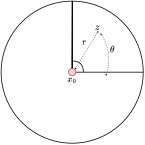
\includegraphics[scale=0.6]{TheorethicalFramework/ND-Laplace/Images/polar-laplace.png}
  \centering
  \caption{Representation of the generated $z = {r \theta}$ and original point $x0$.}
  \label{figure:parea}
\end{figure}

\textbf{Calculating $r$:}
This variable is defined as $dist(x_0, z)$ and can be randomly drawn by inverting the \gls{cdf} for the Laplace distribution:
\begin{equation}
  C{_\epsilon}{^{-1}}(p) = - \frac{1}{\epsilon}(W_-1 (\frac{p - 1}{e}) + 1)
\end{equation}
For this equation, $W_{-1}$ is a Lambert W function with a -1 branch.
\todo[inline]{Explain -1 branch?}
The Lambert w function (also called the product logarithm) is defined as $W(x)e^{W(x)} = x$ \citep{lehtonen_lambert_2016}.
The purpose of the Lambert w function is to invert the \gls{cdf} of the Laplace distribution to generate random noise for one of the coordinates ($r$) using the random value of $p$.

\textbf{Calculating $\theta$:}
The other variable ($\theta$) is defined as a random number $[0, 2\pi]$. \newline
To visualize the data, it is necessary to convert the polar coordinates for $z = (r, \theta)$ back to planar coordinates $z = (x, y)$.
This conversion is described as step 4 of the planar Laplace algorithm \citep{DBLP:journals/corr/abs-1212-1984} and visualized using figure \ref{figure:geo}.
\begin{figure}[h]
  \includesvg[width=0.8\textwidth]{TheorethicalFramework/ND-Laplace/Images/polar-laplace-to-planar.svg}
  \centering
  \caption{Representation of converting the perturbed point $z = (r, \theta)$ to a point ${z_x, z_y}$}
  \label{figure:geo}
\end{figure}

\newpage
\subsection{Truncation} \label{theory:truncation}
After adding the noise to the data, it cannot be ensured the data is within the original domain (figure \ref{figure:truncation-2d}).
If this is not the case, the data is easily distinguished by an unwanted adversary \citep{DBLP:journals/corr/abs-1212-1984,9646489}.
The truncation is an essential part of the mechanism to ensure the data is contained within the domain of the original data $X$.
%We assume a user has a set of data points with a range of [-1, 1].
\begin{figure}[H]
  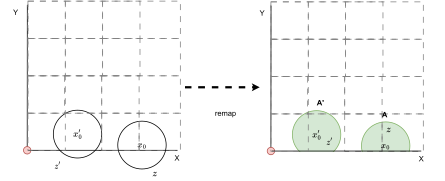
\includegraphics[width=0.7\textwidth]{TheorethicalFramework/ND-Laplace/Images/remapping.png}
  \caption{Representation of truncation of data points for 2-dimensional Laplace mechanism.}
  \label{figure:truncation-2d}
\end{figure}
%A solution was described by Andres et al. in step 5 of the Laplacian mechanism for 2D space \citep{DBLP:journals/corr/abs-1212-1984}.
%A viable solution is to create a grid around the diameter of the set of points $X = R^2$ that belong to the user \citep{DBLP:journals/corr/abs-1212-1984}.
The approach Andres et al. introduces is to remap a perturbed point $z$ to the closest point $x'$ in $G$ \citep{DBLP:journals/corr/abs-1212-1984}.
Here, $G$ is a grid generated using constant cell width.
%Although this approach remaps data within the original domain of $X$, it is not guaranteed it preserves \gls{gi} anymore.
Let the below equation be the collection of probabilities for a point being remapped to a grid cell $x'$ \citep{DBLP:journals/corr/abs-1212-1984}:
\begin{equation}
  R(x) = { y \in R^2 | \forall x' \in G \cdot d(y, x') \leq d(y, x')}
  \label{eq:grid-probability}
\end{equation}
The original \gls{gi} definition contains $K$, which is the probability of $z$ being reported as $x$ (See Equation: \ref{theory:geo-indistinguishability}).
However, this probability is no longer guaranteed because $z$ can also be part of $G$ \citep{DBLP:journals/corr/abs-1212-1984}.
Hence the probability is now $R_X(x) = R(x) \cup X$. \newline
So, the $R_X(x)$ has a different shape depending on the distance $x_0$ and $x'$ (ergo, it depends on the grid cell width). This is due the step units of $G$ stay the same, while the distance $r$ grows \citep{DBLP:journals/corr/abs-1212-1984}.
\newpage
To overcome this issue, Andres et al. propose a way of calculating $\epsilon'$, depending on the step-unit $u$. \citep{DBLP:journals/corr/abs-1212-1984}.
They proved this in theorem 4.1 \citep{DBLP:journals/corr/abs-1212-1984}:
\begin{theorem}[Discretization 2D-Laplace]
  Assume $r_{max} < \frac{u}{\delta_{\theta}}$, and let $q = \frac{u}{r_{max}}\delta_{\theta}$. Let $\epsilon$, $\epsilon' \in R^+$ such that \\
  $\epsilon' + \frac{1}{u}ln \frac{q + 2 e^{\epsilon'u}}{q - 2 e^{\epsilon'u}} \leq \epsilon$ \\
  Then $K_{\epsilon'}$ provides $\epsilon$-geo-indistinguishability within the range of $r_{max}$. Namely, if ${d(x_0, x), d(x'_0, x) \leq r_{max}}$ then: \\
  $K_{\epsilon'}(x_0)(x) \leq e^{\epsilon d(x_0, x'_{0})} K_{\epsilon'}(x'_{0})(x)$.
  \label{theorem:discretization}
\end{theorem}
Here, $\delta_{\theta}$ is the machine's precision, which is the hardware precision of the GPS-location in the context of geographical data. We will omit this in our research, but still provide the full theorem nonetheless. 
The theorem states that $\epsilon'$ is the additional noise needed to satisfy \gls{gi} with the introduction of discretization.
%Then, the final step is truncation based, which is based on the discretization \citep{DBLP:journals/corr/abs-1212-1984}.
It is sufficient to take $r_{max}$ as $diam(X)$, which is the diameter of the set of points $X$ if it satisfies theorem \ref{theorem:discretization} \citep{DBLP:journals/corr/abs-1212-1984}:
So, $r_{max}$ is the maximum distance between points in $X$, which is the area where geo-indistinguishability can be guaranteed \citep{9646489}.

\mycomment{In the context of our research, it is more convenient to find the $u$ based on a given $\epsilon$.
So the challenge is to find the $u$ that satisfies \gls{gi}.
This can be solved by finding the root of the function:
\begin{equation}
  \epsilon' + \frac{1}{u}ln (\frac{\frac{u}{r_{max}} + 2 e^{\epsilon'u}}{\frac{u}{r_{max}} - 2 e^{\epsilon'u}}) - \epsilon = 0
  \label{eq:find-u-with-epsilon}
\end{equation}
The idea of finding the root of a function is to try different values of $u$ until $f(u) = 0$. \todo{Have some proof}
\todo[inline]{Maybe extend this with some more explanation?}}
%This idea was later improved by Chatzikokolakis et al., introducing an optimized way of remapping \citep{chatzikokolakis_efficient_2017}.
%The algorithm uses the Bayesian rule to minimize the loss of utility while remapping the data.
%Instead of remapping to the closest point, it remaps to a location where the loss is minimal.
%To decrease the performance impact of this algorithm, it is possible only to consider a specific region around the perturbed point $z$.
%The disadvantage of this method is the need for a prior set of data points to calculate the optimal remapping.
%It does not work for new users and extends the training period.

\mycomment{\subsection{Optimizing for clustering} \label{2d:optimizing}
The decision of the parameters for the algorithm is straightforward as it depends on the $\epsilon$. \label{paragraph:choosing-r}
This constant is calculated by defining the radius $r$, and the desired level of privacy $l$ and $\epsilon$ is calculated using $l/r$.
The $l$ is a predefined constant $l \in R^+$ but usually will be below 10.
For geographical data, the $r$ can be configured using meters as a unit of measure.
So, for example, $r = 200$ corresponds to a radius of 200m around point $x_0$.
Without a unit, it is a challenge to define a reasonable radius.
%The $\epsilon$ can be considered the inverse unit of $r$ \citep{DBLP:journals/corr/abs-1212-1984}.
In that regard, the radius can also be a flexible value defined based on the crowdedness of a region \citep{chatzikokolakis_constructing_2015}.
Suppose a user's location is within a crowded area.
In that case, the radius can be smaller than if the user is located in a rural area (because the user's location is indistinguishable due to the overlap of other users' locations).
Instead of providing \gls{gi}, the authors introduce a more flexible privacy definition $d_x$-privacy.
The $r$ is calculated based on the mass of other regional locations $r$, which they call \emph{privacy mass}.
So, the total mass of a set A is defined as $M(A) = \sum_{x \in A} m(x) = a + q(x)b$.
Where $m(x)$ is the mass of a location $x$ and $x$ is in value [0, 1].
For this formula, $a$ is the number of points assigned to each location.
The authors define $q(x)$ as the "quality" of a point, which is essentially the number of other users that are also interested in the same point (e.g. a mall).

The $a$ is defined as a Euclidean ball $B_r = {x' | d_{euc}(x, x') \leq r}$, which returns all locations within the radius $r$.
\todo[inline]{Explain this formula better, and create it as a separate equation}
To retrieve a value within [0, 1], the authors use the following formula:
\begin{equation}
  a = \frac{1}{|B_r|}
  \label{equation:privacy-mass-a}
\end{equation}
If the locations are only considered for space and not quality, $q(x)$ is defined as 0 \citep{chatzikokolakis_constructing_2015}.

Although the method is an interesting approach to increasing utility while not reducing privacy, it is hard to adopt for clustering.
For applying it for \gls{ldp}, it is required to supply each user with prior knowledge of the dataset.
This approach would require interaction between data points, hence an interactive setup of the mechanism instead of a non-interactive one. \newline
Nonetheless, the idea of using crowded locations is an exciting approach that is researched further in section \ref{theory:privacy-utility-nd}
}


\newpage
\subsection{Final mechanism}
Finally, we provide as means of a summary the final algorithm for the Laplace mechanism for 2D space
\begin{algorithm}[H]
  \caption{Full mechanism for perturbing training data for planar/2D-Laplace \citep{DBLP:journals/corr/abs-1212-1984}}\label{alg:rq1}
  \begin{algorithmic}
    \Require $X$, $\epsilon$, $u$, $v$ 
    \Ensure $Z$ 
    %\State $r = \frac{\sigma}{2}$ \Comment formula 4.1
    %\State $\epsilon = \frac{l}{r}$ \Comment Calculating privacy budget \citep{DBLP:journals/corr/abs-1212-1984}
    \State Generate $\epsilon'$         \Comment{Theorem: \ref{theorem:discretization}}
    \State $Z \gets \varnothing$
    \State Generate G from given sides $u, v$.
    \State Generate $A$ with acceptable points around $x_0$ 
    \For{$x_i \in X$}
    \State Generate $\theta$       \Comment Equation: \ref{2d:generate-theta}.
    \State Generate the radius $r$ around $x_0$ \Comment Equation: \ref{eq:lambert_w_1}.
    %\State $z_i \gets T(x_{min}, x_{max}, point_i, z_i)$ \Comment algorithm 1.
    \State Convert polar coordinate $(r,\theta)$ to Cartesian coordinates $z = (x, y)$ \Comment Figure: \ref{figure:geo}.
    \If{z $\notin A$}
        \State Remap $z$ to closest point in $A \cap G$. 
    \EndIf
    \State Add $z$ to perturbed set $Z$.
    \EndFor
    \State \Return Z
  \end{algorithmic}
  \label{alg:2d-laplace}
\end{algorithm}
\newpage
\section{3D-Laplace}
The previous sub-section described the use of 2-dimensional noise on geographical data.
This approach has recently been extended to support 3-dimensional data, which benefits indoor navigation \citep{9646489}.
The method is similar to the 2D approach but includes the azimuth angle $\psi$ besides the polar angle $\theta$ and radial distance $r$.

\subsection{Geo-indistinguishability}
To establish the same privacy guarantees for 3-dimensional data as for 2-dimensional data, the original equation \ref{algo:2d-geo-indistinguishability} is extended \citep{9646489}.
\begin{equation}
  K(x_1)(z) \le e^{\epsilon * d_3(x_1, x_2)} K(x_2)(z)
  \label{algo:3d-geo-indistinguishability}
\end{equation}
Where $x_1$ and $x_2$ are two real data points in the same dataset $X$.
%The more $x_1$ and $x_2$ are similar, the more the perturbed location distributions $K(x_1)(z)$ and $K(x_2)(z)$ need to be similar.
\subsection{Spherical Laplace}
The implementation of Min et al. projects the dimensions onto a sphere instead of a circle \citep{9646489}.
This sphere is a unit sphere calculated with a radius of 1.
The polar angle $\theta$ and azimuth angle $\psi$ are randomly calculated based on this sphere. \newline
\textbf{Calculating $\theta$ and $\psi$}: The tuple $U = (\theta, \psi)$ is randomly drawn from the unit sphere using the following equations \citep{9646489}:
\begin{equation}
  \theta = \frac{1}{\pi}
\end{equation}
\begin{equation}
  \psi = \frac{1}{2\pi}
\end{equation}
\textbf{Calculating $r$}: The radial distance $r$ is calculated using the following equation:
\begin{equation}
  r = \frac{1}{2}\epsilon^3 * r^2 * e^{-\epsilon * r}
  \label{eq:3d-laplace-r}
\end{equation}
The gamma scale is the same as for 2D-Laplace but with a shape of 3 instead of 2.
The noise is added to the original location $x$ to obtain the perturbed location $z = x + U*r$.
A clear example of the generated noise by this method is shown in figure \ref{fig:3d-laplace-noise}.
\begin{figure}
  \includegraphics[width=0.6\textwidth]{TheorethicalFramework/ND-Laplace/Images/3d_laplace_noise.png}
  \caption{50 random noise samples generated around point $x_0$ (green dot) using the 3D-Laplace noise method \citep{9646489} plotted on a sphere.}
  \label{fig:3d-laplace-noise}
\end{figure}
Finally, the spherical coordinates are converted to the Cartesian coordinate system to obtain the perturbed location $z$:
\begin{align*}
  z_x = r * \sin(\theta) * \sin(\psi) \\
  z_y = r * \sin(\theta) * \cos(\psi) \\
  z_z = r * \cos(\theta)
\end{align*}
The complete overview is visualized in figure \ref{fig:3d-laplace}.
\begin{figure}
  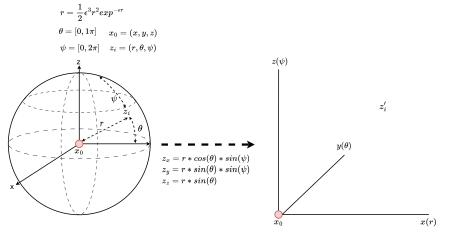
\includegraphics[width=0.8\textwidth]{TheorethicalFramework/ND-Laplace/Images/3d_laplace.png}
  \caption{3D-Laplace noise distribution according to the method proposed by Min et al. \citep{9646489}}
  \label{fig:3d-laplace}
\end{figure}
\newpage
\subsection{Truncation}
As with the 2D-Laplace method, the 3D-Laplace method also needs a truncation method.
This truncation method is also based on the same method as the 2D-Laplace method.
Instead of a plane grid, a cuboid grid is used for 3-dimensional space.
This cuboid remaps the noise to the closest grid cell $g \in G$ or existing point in $X$.
We plotted example data points on a 3-dimensional grid in figure \ref{fig:3d-laplace-example} to demonstrate this:
\begin{figure} [H]
  \includegraphics[width=\textwidth]{TheorethicalFramework/ND-Laplace/Images/example_3d_laplace.png}
  \caption{Applying 3-dimensional noise with $\epsilon = 1$ (red dots) to a dataset $X$ (green dots). Demonstrating remapping to the closest grid point (blue) or $X$.}
  \label{fig:3d-laplace-example}
\end{figure}

\newpage
\subsection{Final mechanism}
Finally, we provide as means of a summary the final algorithm for the Laplace mechanism for 3D space
\todo[inline]{Write down 3D laplace algorithm}
\newpage
\newpage
\section{nD-Laplace}
As mentioned in the previous chapter, the paper that was introduced by Min et al. is be-able to handle 3-dimensional data.
A small recap: a point $(r, \theta, \psi)$ gives us the spherical coordinates of a given 3-dimensional sphere.
An important property for this is the fact that each of these coordinates can be generated separately \citep{DBLP:journals/corr/abs-1212-1984, 9646489}.
The $r$ gives us the radius or distance from $(\theta, \psi)$ to the center of the sphere \footnote{https://mathworld.wolfram.com/SphericalCoordinates.html}.
So, instead of having just these two coordinates, we are be-able to extend this to n-dimensions by considering an n-hypersphere \citep{fernandes_generalised_2019, 9646489}.
To this end, besides points $\theta$ and $\psi$ we also consider $\theta \in S^n$, where S is a unit hypersphere.

The first step to generate the noise is first to select the $r$.
This method is almost identical to the one for 3-dimensional (\ref{eq:3d-laplace-r}).
But, instead of applying a scale of 3, the scale will be $n$ for the number of dimensions in the data \citep{fernandes_generalised_2019}:
\begin{equation}
  \gamma(n, 1/\epsilon)
\end{equation}
For the other dimensions, we consider a vector $U = (\theta_1, \theta_2, \theta_n)$ which is uniformly selected based on a unit $n$-hypersphere $S^n$ \citep{fernandes_generalised_2019}.
We consider the work that was proposed by Marsaglia et al. for 4-sphere that can be used for selecting points from an n-hypersphere \citep{marsaglia_choosing_1972}.
This method resolves around selecting points from a hypersphere by using a uniform distribution for the domain [0, 1].
We adopted the approach that uses the Gaussian distribution \footnote{https://mathworld.wolfram.com/SpherePointPicking.html}.

\subsection{Cartesian coordinates}
As with the 2/3D-Laplace, the spherical coordinates need to be converted to Cartesian to be able to cluster.
It is comparable to the way it was done in the previous chapters, however, as there are an $n$-amount of angles the equation is repeated and slightly different:
\begin{align*}
  x_1 = r * cos (\theta_1)                                          \\
  x_2 = r * sin (\theta_1) * cos (\theta_2)                         \\
  x_{n} = r * sin(\theta_1) … sin(\theta_{n-2}) *cos (\theta_{n-1}) \\
  x_n = r * sin(\theta_{n-1}) * sin(\theta_{n-2}) * sin(\theta_{n-1})
\end{align*}
If we combine sections 1 and 2 of this chapter, we are being able to give a good overview of the solution using a similar image as for the 2D and 3D variants (figure \ref{fig:nd-laplace-overview}).
\begin{figure}[ht]
  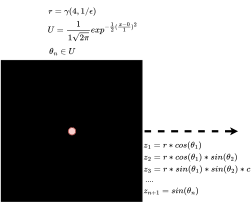
\includegraphics[width=0.6\textwidth]{TheorethicalFramework/ND-Laplace/Images/nd_laplace.png}
  \caption{Overview of the nD-Laplace mechanism}
  \label{fig:nd-laplace-overview}
\end{figure}
\newpage
\subsection{Privacy versus utility} \label{theory:privacy-utility-nd}
If we continue adding dimensions, we notice the noise is shrinking proportionally.
To understand this behavior, we first have to examine the formula for a hypersphere’s volume.
\begin{equation}
  S_n = \frac{2 \pi^{n/2}}{\gamma(\frac{1}{2}n)}
\end{equation}
Where $\gamma$ is the gamma distribution that is determined based on the number of dimensions $n$ \footnote{https://mathworld.wolfram.com/Hypersphere.html}.
As the amount of dimensions increases, the most volume is located on the hypersphere surface.
When we convert the points to Cartesian coordinates, some will be located at the center (e.g., 0.5), while others will be close to the surface (e.g., 0.0).
However, as the number of dimensions increases, the majority will be close to the surface (e.g., 0.99).
The decreasing amount of volume is illustrated using this figure:
\begin{figure}[H]
  \includegraphics[width=0.8\textwidth]{TheorethicalFramework/ND-Laplace/Images/volume.png}
  \caption{Illustration of the decreasing volume while increasing the number of dimensions}
  \label{fig:curse-of-dimensionality}
\end{figure}

The noise decreases as the dimensions increase, increasing utility.
Hence, it is intriguing to observe the behavior of privacy relative to utility.
This behavior will be further emphasized in a later stage of this research.
\newpage
\subsection{Truncation}
For 2D/3D Laplace, a grid and cuboid were respectively introduced to truncate noise mechanisms \citep{DBLP:journals/corr/abs-1212-1984,9646489}.
This section extends the work done for 2D and 3D Laplace (\ref{theory:truncation}, \ref{2d:optimizing}) \newline
This section introduces an extension for handling any number of dimensions, which can also substitute for 2D/3D.
We want to note that this section focuses on improving utility with remapping.
Any remap function preserves geo-indistinguishability \cite{chatzikokolakis_efficient_2017}, so the required privacy is still preserved.

Recalling both mechanisms, the 2D version operates on a plane and approximates on a grid $G$, while the 3D version works in a 3D space using a cuboid grid.
Given a set of input points $X \subset R^2$, we can truncate points that are outside the domain by remapping them to points within $G$ ($Z = X \cap G$) \citep{DBLP:journals/corr/abs-1212-1984}.
Here, $X$ represents other data points reported locally by the same user.
To extend this approach to n-dimensional data, we need an efficient way to search points in an n-dimensional hypersphere.
To do this, we adopt the idea proposed by Chatzikokolakis et al. of using a kd-tree for efficient searching of the grid \citep{chatzikokolakis_efficient_2017}.
In their research, they describe the utilization of a kd-tree for searching nearby points for a given point.
For this reason, we also use a kd-tree for the following tasks:
\begin{enumerate}
  \item Finding nearby points for $z \in G$ (section: \hyperref[theory:grid-remapping]{Grid with kd-tree remapping}).
  \item Finding nearby points for $x \in X$ and $z \in Z$ (section \hyperref[theory:optimal-remapping]{Optimal remapping}).
\end{enumerate}

\subsubsection{Grid with kd-tree remapping} \label{theory:grid-remapping}
A kd-tree is a multidimensional tree of k-dimensions used to store spatial data \citep{bentley_multidimensional_1975}.
Each record is a node in the tree and points to either null or another node.
It is of great interest to our research as it allows for efficient nearest neighbor searching \citep{washington_k-d_2002}.
This enables efficient searching of records based on space. This is illustrated using a two-dimensional representation (figure \ref{fig:kd-tree}).
The biggest benefit of a kd-tree is its efficiency, as its space complexity is $O(kn)$, where $k$ is the number of dimensions and $n$ is the dataset size.
Additionally, nearest neighbor (NN) searching is efficient, with a time complexity of $O(\log n)$ \citep{washington_k-d_2002}.
\begin{figure}[H]
  \includegraphics[width=1\textwidth]{TheorethicalFramework/ND-Laplace/Images/KD-tree.png}
  \caption{Representation of a kd-tree with 2 dimensions to remap based on a grid.}
  \label{fig:kd-tree}
\end{figure}
When using a kd-tree to search for a data point $z_i$, the algorithm begins with an unbalanced binary tree.
The root is split by the x-axis, and since 4.5 is greater than 3.5, we go to the right.
This means that we no longer need to consider the left (greyed out) part of the grid.
We continue traversing the tree until we find the nearest point based on Euclidean distance.

Using this algorithm, we can effectively remap point $z \in Z$ to either $X$ or $G$ based on the closest Euclidean distance (algorithm \ref{alg:grid-remapping-laplace}) and find data points in an n-dimensional space that is outside the original domain (algorithm \ref{alg:find-outside-domain-laplace}).
The utility of this method depends on the number of grid cells in $G$, since a smaller distance will result in more frequent mapping to the surface of the grid.
When $\epsilon$ is very low (and thus closer), the data points are more likely to map to the grid surface (\ref{fig:3d-laplace-noise}, \ref{fig:3d-laplace-example}).
Increasing the number of grid cells can improve the utility, but this comes at the cost of significantly increased space complexity for $k$ dimensions.
This is because a grid of $n*m$ dimensions has a complexity of $O(n^2)$.
Therefore, we also explore the optimal remapping algorithm proposed by Chatzikokolakis et al \citep{chatzikokolakis_efficient_2017}.
\begin{algorithm}[H]
  \caption{Algorithm for finding points outside the domain of $X$.}
  \begin{algorithmic}
    \Require $x \in X$  \Comment original dataset
    \Require $z \in Z$ \Comment perturbed dataset
    %\State $tree \gets KDTree(X)$ \Comment construct a KDTree from the original data.
    \State $X_{domain} \gets \Call{KDTree::query}{Z}$ \Comment find the closest points.
    \State $X_{features} \gets \Call{List::getfeatures}{X}$ \Comment retrieve dataset dimensions
    \State $X_{outside-domain} \gets []$
    \For{$feature \in X_{features}$} \Comment iterate over all features and check if any points are outside the domain.
    \If{$feature \leq \Call{X::min}{Z} $}
    \State $\Call{row::append}{X_{outside-domain}}$
    \EndIf
    \If{$feature \geq \Call{X::max}{Z} $}
    \State $\Call{row::append}{X_{outside-domain}}$
    \EndIf
    \EndFor
    \State \Return $X_{outside-domain}$ \Comment The index of points outside the domain of $X$.
  \end{algorithmic}
  \label{alg:find-outside-domain-laplace}
\end{algorithm}
\begin{algorithm}[H]
  \caption{Algorithm for generating and remapping to a grid.}
  \begin{algorithmic}
    \Require $x \in X$  \Comment n-dimensional array of original points

  \end{algorithmic}
  \label{alg:grid-remapping-laplace}
\end{algorithm}

\subsubsection{Optimal remapping} \label{theory:optimal-remapping}
As we discussed, the remapping will be performance intensive and that is why we adopt the optimal remapping \citep{chatzikokolakis_efficient_2017}.
Consider the grid that was proposed in \ref{fig:kd-tree}.
After remapping point $z_i$, it is mapped to the center for the grid cell.
Based on the cell width, the distance to the original point $x_i$ and $ z_i$ could be really large.
Therefore, it is more efficient to remap in the following way:
\begin{figure}[H]
  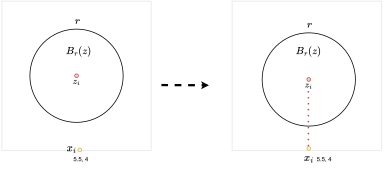
\includegraphics[width=0.7\textwidth]{TheorethicalFramework/ND-Laplace/Images/optimal-remapping.png}
  \caption{Representation of optimal remapping \citep{chatzikokolakis_efficient_2017}, where $z_i$ is remapped to $x_i$ using $\sigma(x)$ instead of the center of the grid cell.}
  \label{fig:optimal-remapping}
\end{figure}
The remapping algorithm works on the idea of crowded places \ref{2d:optimizing}, with the intuition that a crowded place leverages indistinguishability by crowdedness.
This works by considering a prior set of data point $Q \in R^n$.
Which are other data points that belong to the user.
We are interested in the data points that are within the radius $r$ around $z$.
This is denoted as $B_r(z)$, which is the vector of all points within radius $r$ around $z$.
In addition to this, there is also a $Q_r$ that is a convex hull of all nearby points.
Hence, this is described as $Q_r = B_r \cap Q$.
The final intuition here is that $r$ is automatically generated based on crowdedness (see circle inside figure \ref{fig:optimal-remapping}).

The first step is to assign weights $w(q) $ to each data point in $Q_r$, which is described by Chatzikokolakis et al. as the “popularity” of a prior location $q$.
Because we do not consider locations (where points of interest are fixed coordinates) we are not able to get an accurate count for $w(q)$.
Therefore, we re-use equation 3.4 and define $ w(x)$ as $ |Q_r|$ and use kd-tree again to efficiently find $|Q_r|$.
The second step revolves around calculating $\sigma(x)$:
\begin{equation}
  \sigma(x) = \frac{w(x)e^{-\epsilon d(x, z)}}{\sum{_{q\in Q_r} w(q)e^{-\epsilon d(q, z)}}}
  \label{eq:optimal-remapping-formula-1}
\end{equation}
The last step is to take the mean value of $\sigma(x)$.
Unfortunately, optimal remapping is not possible for users that do not have sufficient data (e.g. new users).
The remapping is not applied for these users and is also not applied for $z$ if it is within the domain of $X$.

\subsubsection{Practical implementation}
For practical implementation, we will consider $Q_r$ as a set of locations within a radius $r$ of $z$.
As explained in the previous paragraph, it is difficult to interpret $w(q) \in Q_r$ because we cannot calculate "crowded" places.
Therefore, we interpret $w(q)$ as a simple count of all data points within $Q_r$ excluding $z$. Calculating $z'$ using $\sigma(x)$ is easier:
\begin{equation}
  \sigma(x) = \frac{w(x)e^{-\epsilon d(x, z)}}{w(q)e^{-\epsilon d(q, z)}}
  \label{eq:optimal-remapping-formula-2}
\end{equation}
So, $w(x) = 1$ and $w(q)$ is the count of all locations except $x$ and $z$. It is also not necessary anymore to calculate the mean.

It is also possible to implement equation \ref{eq:optimal-remapping-formula-1} without any modifications.
This requires us to implement the mechanism interactively.
In this approach, all clients perturb their data and sent it to the server.
The server clusters the private data and calculates weight based on cluster information (e.g., crowdedness/density) and shares it with the clients.
The clients then use the optimal remap and share their private information with the server again.
Although this system requires only a single round-trip between server and clients \todo {Add link to figure next section}, it reveals cluster information, so we prefer the non-interactive setup (\todo{Add link to figure next section}).

\begin{algorithm}[H]
  \caption{Algorithm to implement the density remapping of $Z$ to be in the domain of $X$}
  \begin{algorithmic}[1]
    \Require $X, Z, \epsilon$                                \Comment{Requires a truncated nD-Laplace output $Z$}
    \Ensure $Z'$
    \State Filter $Z$ with the data points that were remapped by grid.
    \State Construct a kd-tree from $X$
    \For{$z \in Z$, $x, r \in X$}
    \State Find all points $X_r$ inside radius $r$  around $x$ 
    \State Find all points $B_r$ inside radius $r$ around $z$
    \State $\sigma(x) = []$
    \State $Q_r = X_r \cap B_r$
    \State Count number of points $w_r$ within $Q_r$
    \For{$q \in Q_r$}
    \State Find all points $q$ inside radius $r$ around $q$.
    \State Count number of points $w_q$ within $q$.
    \State Calculate $\sigma(x)$ \Comment Equation \ref{eq:optimal-remapping-formula-1}.
    \State Add $\sigma(x)$ to list
    \EndFor
    \State Calculate $z'$ using $Q_r$ and $\sigma(x)$ \Comment Equation: \ref{eq:optimal-remapping-formula-2}.
    \EndFor
  \end{algorithmic}
  \label{alg:optimal-remapping-laplace}
\end{algorithm}

\begin{itemize}
  \item 1: Receives all the points $z \in Z$ that were originally outside the boundary of $X$ (before remapping).
  \item 2: Constructs a KDTree from the original data $X$, so it can be queried.
  \item 6: Denotes the list of densities for point $x$.
  \item 7: Holds the data-points within the radius $r$ of both $x$ and $z$.
\end{itemize}



\subsection{Putting it together}
\todo[inline]{Create algorithm for nD-Laplace}
\begin{algorithm}[H]
   \caption{Full algorithm for perturbing training data for nD-clustering using nD-Laplace}
   \begin{algorithmic}
      \Require $x \in X$  \Comment n-dimensional array of original points
      \Require $\epsilon$ \Comment privacy budget
      \Ensure $z \in Z$ \Comment n-dimensional array of optimal-remapped perturbed points
      \State $sphere = \Call{GenerateUnitSphere}{x}$ \Comment construct a sphere around $x$.
      \For{$row \in X$}
      \State $d \gets \Call{Length}{row}$ \Comment amount of dimensions
      \State $r \gets \Call{GenerateRadius}{d}$ \Comment Equation \ref{eq:generate_r_for_nd_laplace}.
      \State $sphere \gets \Call{GenerateTheta}{d}$ \Comment Equation \ref{eq:generate_theta_for_nd_laplace}.
      \State $noise \gets \Call{Cartesian}{row, \epsilon}$ \Comment Equation \ref{eq:nd-laplace-cartesian}.
      \State $z = x + noise$
      \State \Call{Append}{$Z, z$}
      \EndFor
      \State \Return Z
   \end{algorithmic}
   \label{alg:nd-laplace}
\end{algorithm}
%\subsection{Extending to $d_x$-privacy}
%\todo[inline]{Find if this is possible}

%Constructing elastic distinguishability metrics for location privacy
\newpage

\subsection{Mechanism overview}
In conclusion, the nD-Laplace mechanism is capable of providing $\epsilon-d_x$-privacy (as well as \gls{gi}) as demonstrated in Formula \ref{theorem:nd-laplace}. The grid-nD-Laplace variant also offers the same privacy guarantee, as proven in Section \ref{section-grid-remapping}. Additionally, the density-nD-Laplace mechanism, being a post-processing step, provides an equivalent level of privacy as nD-Laplace. This equivalence extends to clustering as well \citep{feyisetan_leveraging_2019}.

Furthermore, it is worth noting that the use of kd-trees simplifies the complexity of these variants without compromising their privacy guarantees. Kd-trees serve as a tool to address the search complexity in handling n-dimensional data, rather than directly affecting the privacy assurances.
The following sections will provide a comprehensive framework overview and offer practical insights for its application.

\subsubsection{Flowchart}
All formulas and theories are established for 2D-Laplace, 3D-Laplace, and nD-Laplace, so the mechanism design applies to all three variants:
\begin{figure}[H]
  \includegraphics[width=1.1\textwidth]{TheorethicalFramework//ND-Laplace//Images/overview.png}
  \caption{Non-interactive mechanism design for nD-Laplace.}
  \label{fig:final-mechanism-design}
\end{figure}
%\todo[inline]{Modify to density-nD-Laplace \& nD-Laplace for image reporting}
For easy navigation, we provide a list of all algorithms:
\begin{enumerate}
  \item Based on the number of dimensions, the algorithm decides the correct Laplace mechanism to use:
        \begin{itemize}
          \item 2D-Laplace:  Algorithm: \ref{alg:2d-laplace}
          \item 3D-Laplace:  Algorithm:\ref{alg:3d-laplace}
          \item nD-Laplace: Algorithm: \ref{alg:nd-laplace}
        \end{itemize}
  \item Grid remapping: Section:\ref{section-grid-remapping}
  \item Density remapping: Algorithm: \ref{alg:optimal-remapping-laplace}
\end{enumerate}
In addition, relevant research questions are incorporated into the architecture overview.
These questions are covered in chapter \ref{chapter:methodology}.
\subsubsection{Practical example}
The shape of the dataset is necessary for the usefulness of clustering.
With our algorithm, there are four different shapes/variants of the dataset.
For example, this has been visualized using a 2D dataset based on the Circle dataset (\ref{datasets-section}).
Our mechanism aims to provide privacy and preserve the dataset its shape to benefit the utility of clustering.
Grid remapping and density remapping are used to achieve this goal.

\begin{figure}[H]
  \includegraphics[width=1.1\textwidth]{TheorethicalFramework//ND-Laplace//Images/output.png}
  \caption{Example of optimal remapping for the 2-dimensional Circle dataset. The example shows the different steps of the mechanism in sequence for a dataset perturbed with a privacy budget of 0.5.}
\end{figure}
\begin{enumerate}
  \item Dataset: the blue dots represent the original dataset without any modifications.
  \item Adding noise: the green crosses represent the dataset after adding noise; for this particular example, this is 3D-Laplace (Algorithm \ref{alg:3d-laplace}):
        As can be observed, the data is generated from the center, causing many data points to fall outside the original domain of the dataset.
  \item Grid-remapping: the red dots represent the dataset after grid-remapping (Section \ref{section-grid-remapping}).
        After performing the grid remapping algorithm, all points outside the data domain are remapped to be within the domain. The data-shape is also partly restored. 
  \item Optimal-remapping: the green dots represent the dataset after optimal-remapping (Algorithm \ref{alg:optimal-remapping-laplace}). As can be observed, this process is primarily focused on achieving a better utility by reproducing the original shape.
\end{enumerate}

